\section{Parsing}
\label{sec:parsing}

The parser is responsible to generate the LTAG/DUDES representation of a question expressed in natural language\footnote{we have restricted our research to the English language.}. 
%
The parser takes in input a natural language sentence $S$, the grammar $G$ and the ontology $O$ \footnote{as stated in the previous sections, we assume that $G$ is aligned to $O$ through a lexicon.}.
%
In particular, it leverages $G$ to recognize lexical entries in $S$, and $O$ to execute reasoning steps for disambiguation during parsing.
%
The generated DUDES is finally used by the application control layer to compose the SPARQL query to be submitted to the ontology.


The parser has been designed addressing two main requirement: \textit{correctness} and \textit{limitation of the syntactic/semantic search space}, which is the most critical aspect to achieve better performance.
%
The previous requirements have been met through a parsing algorithm that is (i) deterministic (ii) greedy and (iii) particularly focused on structural aspects of LTAG.
Furthermore, the performance boost in terms of response-time have been achieved though the limitation of the interaction with the ontology.

The parsing process is carried out by two main functional components: 
(i) the \texttt{Tokenizer}, which recognizes in the sentence textual patterns that can be traced back to grammar entries, and sequentially emit them as tokens, and 
(ii) the \texttt{Parser} itself, which consumes these tokens, composing them to make LTAG/DUDES compositions\footnote{both substitutions and adjunctions.}.

In Section~\ref{sec:parsing-tokenization} and Section~\ref{sec:parsing-algorithm} we describe and motivate the architectural choices and the pseudocode realizing tokenization and the parsing algorithm, respectively.
%
Furthermore, in Section~\ref{sec:parsing-ambiguities} and Section~\ref{sec:parsing-support-dudes-composition} we show how our parser solve ambiguities through reasoning and how it supports DUDES composition though main variables mappings.

\subsection{Tokenization}
\label{sec:parsing-tokenization}

Given a grammar $G$ and a sentence $S$, the tokenization phasepartitions $S$ in a ordered sequence of regular expressions $\{\pi\}$, each one referring at least one elementary LTAG/DUDES in $G$.
%
The \texttt{Tokenizer} is the software component responsible to execute the tokenization pahse.

In Figure~\ref{fig:tokenizer-sample} we show some notable execution of the tokenization phase.
%
Every time the \texttt{Tokenizer} is invoked on $S$ with $G$, it looks in $S$ for the \textit{longest regular expression} matching an entry in $G$.
%
Once the regular expression has been matched, the \texttt{Tokenizer} emits a \textit{token} $t$, that is an element defined as follows:

\begin{equation}
\label{eqn:token}
token:=(regexp,pos,candidates)
\end{equation}

where
$regexp$ is the regular expression matched in the substring of $S$ starting at position $pos$, and
$candidates$ is the list of LTAG/DUDES in $G$ associated with $regexp$.

Notice that $pos$ is recorded inside a token because it can be used by the parsing algorithm to always be able to locate a token inside the sentence.

\begin{figure}[tp]
	\centering
	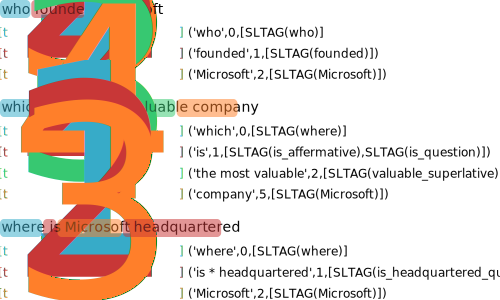
\includegraphics[width=0.8\columnwidth]{./fig/tokenizer-sample}
	\caption{An example of the tokenization phase. In this figure, we denote with \textit{LTAG/DUDES('word')} the elementary LTAG/DUDES associated to the entry \textit{'word'}.}
	\label{fig:tokenizer-sample}
\end{figure}

The \texttt{Tokenizer} is stateful component, hence it leverages convenient data structures to incapsulate its state.
%
The most important one is the \texttt{TokenizerBuffer}, that records whether or not a word in $S$ has been already tokenized.

In Algorithm~\ref{alg:tokenizer} we show the pseudocode of the tokenization process.
%
The \texttt{Tokenizer} exposes a convenient API to iterate over tokens, that is clearly inspired to the well known API provided by Java generic iterators.

\begin{algorithm}[t]
	\SetKwProg{Fn}{Function}{}{}  
	%\Fn{nextTokenizable()}{
	%\For{$b\in buffer$}{
	%	\If{$b.tokenizable\; \& \; b.tokenized$}{
	%		\KwResult{$buffer.index(b)$}
	%	}
	%}
	%\KwResult{$-1$}
	%}	
	
	\Fn{hasNext()}{
	%\KwResult{$nextTokenizable() \neq -1$}
	}
	
	\Fn{next()} {
		$start \leftarrow nextTokenizableIndex()$ \\
		\If{$\neg start1$}{
			\KwResult{$NULL$}
		}
	
		$end \leftarrow start$ \\
		
		\While{$end < buffer.size$}{
			$elem \leftarrow buffer.get(end)$ \\
			\If{$elem.tokenized = False$}{
				$tmpRegexp.concat(elem.word)$ \\
			}
			$matchType \leftarrow grammar.matchMode(tmpRegexp)$ \\
			\If{$matchType = FULL$}{
				$candidates \leftarrow grammar.getAll(tmpRegexp)$ \\
				$regexp \leftarrow tmpRegexp$ \\
				$buffer.get(end).tokenized \leftarrow True$ \\
				\If{$returnFirstFull = True$}{
					break
				}
			}
			\ElseIf{$matchType = NONE$}{
				break
			}
			\ElseIf{$matchType = PART$}{
				$buffer.get(end).tokenized \leftarrow True$ \\
			}
			\ElseIf{$matchType = STAR$}{
				\If{$consuming = False$}{
					$consuming \leftarrow True$ \\
					$startConsuming \leftarrow end$ \\
				}
				\Else{
					\If{$end = buff.size - 1$}{
						$consuming \leftarrow False$ \\
						$end \leftarrow startConsuming - 1$ \\
						$returnFirstFull \leftarrow True$ \\
					}
				}
			}
		
			$end \leftarrow end + 1$ \\
		}
	
		\KwResult{$Token(regexp,pos,candidates)$}		
	}
	\caption{Pseudocode of the \texttt{Tokenizer} API.}
	\label{alg:tokenizer}
\end{algorithm}

Some functions in Algorithm~\ref{alg:tokenizer} have not been formally defined because they are pretty self-explanatory or have been partially introduced in previous sections.
For reader's sake, we briefly describe the most important ones here. 

Recall that an entry $e$ in grammar $G$ is a tuple

\begin{equation}
\label{eqn:grammar-entry}
e:=(regexp,LTAG/DUDES)
\end{equation}

where
$regexp$ is the regular expression representing the syntactic usage of $e$ in a sentence, and
$LTAG/DUDES$ is the elementary LTAG/DUDES in $G$ representing the syntax and semantics of $e$.

\texttt{grammar.matchMode(str)} matches the specified string str against the entries in grammar. 
%
The following matching modes have are defined:
%
\begin{itemize}
	\item[FULL] the grammar contains an entry matching str, and no entry starting with it. 
	For example, the entry \textit{'Microsoft'} matches is such way the grammar $\{who,founded,Microsoft\}$.
	
	\item[PART] the grammar contains no entry matching str, but an entry starting with it.
	For example, the entry \textit{'founders'} matches is such way the grammar $\{who,are,the,founders of,Microsoft\}$.
	
	\item[STAR] the grammar contains no entry matching str, but a entry starting with it and consuming the last part of it with the \textit{star-operator (*)}.
	For example, the entry \textit{'is'} matches is such way the grammar $\{where,is\;*\;headquartered,Microsoft\}$.

	\item[NONE] the grammar contains no entry matching str in one of the previous mode.
	For example, the entry \textit{'Google'} matches is such way the grammar $\{who,founded,Microsoft\}$.
\end{itemize}

\texttt{grammar.getAll(entry)} retrieves from the grammar all the SLTAGs associated with a regular expression matching the entry in \texttt{FULL} mode.
\subsection{Parsing Algorithm}
\label{sec:parsing-algorithm}

The parser we propose adopts an algorithm aiming to reduce the syntactic/semantic search space and response-time of the parsing process.
%
The search space reduction is achieved by the adoption of a greedy approach, consuming tokens left-to-right and eventually buffering ambiguities.
%
The response-time reduction is achieved by the limitation of the interaction with the ontology during the parsing process. 
%
Such a limitation is achieved by limiting the ambiguity resolution process to those candidates that are strictly semantically ambiguous.
%
In fact, all candidates that are infeasible due to their LTAG structure are excluded before the ambiguity resolution step. 

The parser is a stateful component, hence it leverages convenient data structures to encapsulate its state.
%
The parser state is defined as follows:

\begin{equation}
\label{eqn:parser-state}
	\Sigma:=(words,position,main,waitBuff,ambiguityBuff)
\end{equation}

where
\textit{words} is the list of words in the sentence,
\textit{position} is the current parsing position in the sentence,
main it the current working LTAG/DUDES ($S$-rooted),
\textit{waitBuff} is the data structure that buffers LTAG/DUDES that are not ambiguous, but are waiting to be composed with the $main$ and 
\textit{ambiguityBuff} is the data structure that buffer ambiguous LTAG/DUDES.

In Algorithm~\ref{alg:parser} we show the pseudocode of the parsing process.
%
The \texttt{Parser} exposes a very simple API, made up of only one function.

\begin{algorithm}[t]
\label{alg:parser}
\SetKwProg{Fn}{Function}{}{}  

\Fn{parse (grammar,ontology,question)} {
	$state \leftarrow new\; ParserState(question)$ \\
	$tokenizer \leftarrow new\; Tokenizer(grammar,question)$ \\
	
	\While{$token = tokenizer.next()$}{
		$candidates \leftarrow token.candidates$ \\
		\If{$candidates.isEmpty()$}{
			Error(Cannot find suitable LTAG/DUDES for lexical pattern)
		}
		\If{$candidates.size > 1$}{
			filterAmbiguities(state,candidates,ontology)
		}
	
		\If{$candidates.size = 1$}{
			$candidate \leftarrow candidates.get(0)$ \\
			\ElseIf{$isSentence(candidate)$}{
				\If{$\neg state.curr = NULL$}{
					Error(multiple sentence root found) \\
				}
				$state.curr \leftarrow candidate$ \\
			}
			\Else{
				produce(state,candidate)
			}
		}
	
		\If{$\neg state.curr = NULL$}{
			consume(state) \\
		}		
	}

	\If{$state.curr = NULL$}{
		Error(Cannot build LTAG/DUDES)
	}
	
	\For{$ambiguity \in state.ambiguities$}{
		solveAmbiguity(state,ontology,ambiguity) \\
	}

	$state.curr.semantics.isSelect \leftarrow \neg isAskSentence(question)$ \\
	
	\KwResult{$curr$}
}
\caption{Pseudocode of the \texttt{Parser} API.}
\end{algorithm}

Some functions in Algorithm~\ref{alg:parser} have not been formally defined because they are pretty self-explanatory or have been partially introduced in previous sections.
%
For reader's sake, we briefly describe the most important ones here.
%
The function \texttt{isAskSentence(question)} checks if the given \textit{question} should produce an ASK SPARQL query, rather than a SELECT one. It returns true if the question starts with one of the following words: \textit{do,does,did,am,is,are,was,were}.
%
The function \texttt{isSentence(candidate)} checks whether or not the given SLTAG \textit{candidate} has an LTAG rooted in the \textit{S syntax category}.

The function \texttt{filterAmbiguities(state,candidates)} is called when multiple elementary LTAG/DUDES has been found for the given lexical entry.
%
Given the set of candidates, it leverages the current parser state to filter out those that are not feasible due to their LTAG structure.
%
All those candidates that cannot be filtered out in such a way are considered semantically ambiguous and are buffered to be solved later on.

The function \texttt{produce(state,candidate)} adds the given LTAG/DUDES \textit{candidate} to the parser queue. Such a queue is useful to buffer those LTAG/DUDES that cannot be processed until a S-rooted LTAG/DUDES has been found.
%
The function \texttt{consume(state)} consumes the buffered candidates, composing them with the current main LTAG/DUDES. The combination gives an higher priority to candidates for substitution with respect to candidates for adjunctions.

The function \texttt{solveAmbiguity(state,ontology,ambiguity)} solves the remaining semantic ambiguities. In Section~\ref{sec:parsing-ambiguities} we go into details of the ambiguities resolution process.
\subsection{Ambiguities}
\label{sec:parsing-ambiguities}

When a sentence contains a lexical entry that corresponds to multiple elementary LTAG/DUDES in grammar, we say that an \textit{ambiguity} is occurring.
%
A \textit{syntactic ambiguity} occurs when an entry corresponds to multiple elementary LTAG/DUDES with different LTAG
%
A \textit{semantic ambiguity} occures when and entry corresponds to multiple elementary LTAG/DUDES, with same LTAG and different DUDES.
%
Typically, a syntactic ambiguity is easier to solve than a semantic one, because the former can be solved by structural analysis of LTAG, while the latter needs some resoning steps.

In our solution, we solve both form of ambiguities.
%
In particular, when ambiguities arise, the colliding LTAG are structurally analyzed to filter out all syntactic ambiguities.
%
All semantic ambiguities are solved by checking the consistency of their DUDES with respect to the given ontology.

In Figure~\ref{fig:ambiguities-1} and Figure~\ref{fig:ambiguities-2} we give an example of ambiguities resolution.
%
Let us consider the question \textit{'Is Satya Nadella italian?'}. Here we have the following ambiguities:

\begin{itemize}
\item the entry \textit{'is'} induces a syntactic ambiguity because it corresponds to the elementary LTAG/DUDES with LTAG (a) and (b).
%
The ambiguity is solved by excluding (a), because it contains a substitution node on the left of the lexical entry, hence it cannot suitable to parse the first word of a sentence. 
%
Finally, (b) is considered as to be the only feasible LTAG/DUDES.

\item the entry \textit{'italian'} induces a syntactic/semantic ambiguity because it corresponds to the elementary LTAG/DUDES with LTAG (c)/(d) and DUDES (e)/(f).
%
The ambiguity is solved in two steps.
%
First, the LTAGs (d) with DUDES (e) and (f) are excluded because they cannot be adjuncted to the main LTAG/DUDES.
%
Then, (f) is excluded because the proposition \textit{hasHeadquarter(x,y)} cannot have domain \textit{Person} as the entry `Satya Nadella` has.
%
Finally, the LTAG (c) with DUDES (e) is considered as to be the only feasible LTAG/DUDES.
\end{itemize}

\begin{figure}[tp]
\caption{An example of syntactic ambiguity resolution. Ambiguous LTAG for the entry \textit{'is'}.}
\label{fig:ambiguities-1}
	\begin{tabular}{ p{10em} p{10em} }
		\begin{center}
			(a)
			\begin{tikzpicture}
			\Tree [.S [.DP$_1\downarrow$ ] [.VP [.V is ] [.DP$_2\downarrow$ ] ] ]
			\end{tikzpicture}
		\end{center}		
		&
		\begin{center}
			(b)
			\begin{tikzpicture}
			\Tree [.S [.VP [.V is ] [.DP$_1\downarrow$ ] ] [.DP$_2\downarrow$ ] ]
			\end{tikzpicture}
		\end{center}
	\end{tabular}
\end{figure}

\begin{figure}[tp]
\caption{An example of syntactic/semantic ambiguity resolution. Ambiguous LTAG/DUDES for the entry \textit{'italian'}.}
\label{fig:ambiguities-2}
\begin{tabular}{ p{10em} p{10em} }
	\begin{center}
	(c)
	\begin{tikzpicture}
	\Tree [.DP [.ADJ italian ] ]
	\end{tikzpicture}
	\end{center}		
	&
	\begin{center}
	(d)
	\begin{tikzpicture}
	\Tree [.NP [.ADJ italian ] [.NP* ] ]
	\end{tikzpicture}
	\end{center}		
	\\
	\begin{center}
	(e)
	\begin{tabular}{|c|l|}
		\hline
		\mbox{x} & \\ 
		\hline
		\multicolumn{2}{|l|}{
			$hasNationality(x,y)$
		}\\
		\multicolumn{2}{|l|}{
			$y=Italy$
		}\\
		\hline
		\multicolumn{2}{|l|}{
			\mbox{}
		}\\
		\hline
	\end{tabular}
	\end{center}
	&
	\begin{center}
	(f)
	\begin{tabular}{|c|l|}
		\hline
		\mbox{x} & \\ 
		\hline
		\multicolumn{2}{|l|}{
			$hasHeadquarter(x,y)$
		}\\
		\multicolumn{2}{|l|}{
			$y=Italy$
		}\\
		\hline
		\multicolumn{2}{|l|}{
			\mbox{}
		}\\
		\hline
	\end{tabular}
	\end{center}	
\end{tabular}
\end{figure}

Our parse leverages a reasoning step to solve semantic ambiguities.
%
Whenever a semantic ambiguities arise, a SPARQL query is generated from the DRS statements of each ambiguous DUDES to test its feasibility.

In the following Figures~\ref{fig:ambiguities-resolution-a}-\ref{fig:ambiguities-sparql} we can see an example.
%
Let us consider the main LTAG/DUDES (a) and the ambiguous LTAG/DUDES.
%
The feasibility of DUDES in (b) with respect to (a) is tested by the SPARQL query in Figure~\ref{fig:ambiguities-sparql}. Since the query returns True only for the second DUDES, the first one is excluded.

\begin{figure}[tp]
\caption{An example of ambiguity resolution through reasoning. The main LTAG/DUDES (a)}
\label{fig:ambiguities-resolution-a}
\begin{tabular}{ p{10em} p{10em} }
	\begin{center}
	\begin{tikzpicture}
	\Tree [.S [.VP [.V is ] [.DP$_1$ Microsoft ] ] [.DP$_2\downarrow$ ] ]
	\end{tikzpicture}
	\end{center}		
	&
	\begin{center}
	\begin{tabular}{|c|l|}
		\hline
		\mbox{} & x y \\ 
		\hline
		\multicolumn{2}{|l|}{
			$x=Microsoft$
		}\\
		\multicolumn{2}{|l|}{
			$x=y$
		}\\
		\hline
		\multicolumn{2}{|l|}{
			\mbox{$(y,DP_2)$}
		}\\
		\hline
	\end{tabular}
	\end{center}
\end{tabular}
\end{figure}

\begin{figure}[tp]
\caption{An example of ambiguity resolution through reasoning. The LTAG/DUDES that must be checked for semantic feasibility (b)}
\label{fig:ambiguities-resolution-b}
\begin{tabular}{ p{10em} p{10em} p{10em} }
	\begin{center}
	\begin{tikzpicture}
	\Tree [.DP [.ADJ italian ] ]	
	\end{tikzpicture}
	\end{center}		
	&
	\begin{center}
	\begin{tabular}{|c|l|}
		\hline
		\mbox{x} & x y \\ 
		\hline
		\multicolumn{2}{|l|}{
			$hasNationality(x,y)$
		}\\
		\multicolumn{2}{|l|}{
			$y=Italy$
		}\\
		\hline
		\multicolumn{2}{|l|}{
			\mbox{}
		} \\
		\hline
	\end{tabular}
	\end{center}
	&
	\begin{center}
	\begin{tabular}{|c|l|}
		\hline
		\mbox{x} & x y \\ 
		\hline
		\multicolumn{2}{|l|}{
			$hasHeadquarter(x,y)$
		}\\
		\multicolumn{2}{|l|}{
			$y=Italy$
		}\\
		\hline
		\multicolumn{2}{|l|}{
			\mbox{}
		} \\
		\hline
	\end{tabular}
	\end{center}	
\end{tabular}
\end{figure}

\begin{figure}[tp]
\caption{An example of ambiguity resolution though reasoning. The SPARQL query to test semantic feasibility for ambiguity in Figure~\ref{fig:ambiguities-resolution-b}.}
\label{fig:ambiguities-sparql}
\begin{center}
\begin{verbatim}
ASK WHERE {
    :Microsoft rdf:type ?class1 . 
    :Italy rdf:type ?class2 . 
    hasNationality rdfs:domain ?class1 . 
    hasNationality rdfs:range ?class2
} 
\end{verbatim}	
\end{center}
\end{figure}
\subsection{Support to DUDES composition}
\label{sec:parsing-support-dudes-composition}

In this section we show how our parser supports DUDES composition though \textit{main variable mappings}.
%
First of all, we state here some useful definitions.
%
An \textit{obfuscated variable} is a main variable of a DUDES that is lost at time $t_{1}$ due to substitution, though it should be referenced by some other DUDES at time $t_{2}>t_{1}$.
%
We call \textit{obfuscating substitution} a DUDES substitution that creates an obfuscating variable.

In Figure~\ref{fig:obfuscating-substitution-1} we show an example of obfuscating substitution. 
%
Let us consider the question \textit{'did Microsoft acquire an italian company?'}.
%
We have the main LTAG/DUDES (a), the waiting LTAG/DUDES (b) and the ambiguous LTAG/DUDES (c).
%
The substitution of (b) in (a) is an obfuscating substitution, because once executed, the resulting main LTAG/DUDES in Figure~\ref{fig:obfuscating-substitution-2}.
%
Notice that the resulting main LTAG/DUDES does not have the main variable any more, due to the normal DUDES substitution.
%
Such a situation makes the adjunction of (c) loose its semantic value, due to the absence of the main variable.

Our parser overcome this limitation by detecting obfuscating substitutions. 
%
In particular, it records obfuscated variable, making them accessible by successive adjunctions.
%
In this way, the semantic value of (c) would have never been lost.
%
When (c) is processed, the parser detects that it is looking for an obfuscated variable and makes it temporaly available in the semantics of the main LTAG/DUDES.
%
Once the obfuscated variable have been used, it will never be considered any more.

\begin{figure}[H]
	\caption{An example of obfuscating substitution (a),(b),(c).}
	\label{fig:obfuscating-substitution-1}
	\begin{tabular}{ p{10em} p{10em} p{10em} }
		\begin{center}
		(a)
		\begin{tikzpicture}
			\Tree [.S [.V did ] [.S [.DP  Microsoft ] [.VP [.V acquire ] [.DP [.DET a ] [.NP$\downarrow$ ] ] ] ] ]
		\end{tikzpicture}
		\end{center}		
		&
		\begin{center}
		(b)
		\begin{tikzpicture}
			\Tree [.NP company ]	
		\end{tikzpicture}
		\end{center}		
		&
		\begin{center}
		(c)
		\begin{tikzpicture}
			\Tree [.NP [.ADJ italian ] [.NP* ] ]
		\end{tikzpicture}
		\end{center}		
		
		\\
			
		\begin{center}
		\begin{tabular}{|c|l|}
		\hline
		\mbox{} & x y \\ 
		\hline
		\multicolumn{2}{|l|}{
			$isAcquiredBy(x,y)$
		}\\
		\multicolumn{2}{|l|}{
			$y=Microsoft$
		}\\
		\hline
		\multicolumn{2}{|l|}{
			\mbox{$(x,NP)$}
		} \\
		\hline
		\end{tabular}
		\end{center}
		&
		\begin{center}
		\begin{tabular}{|c|l|}
		\hline
		\mbox{x} & x \\ 
		\hline
		\multicolumn{2}{|l|}{
			$Company(x)$
		}\\
		\hline
		\multicolumn{2}{|l|}{
			\mbox{}
		} \\
		\hline
		\end{tabular}
		\end{center}	
		&
		\begin{center}
		\begin{tabular}{|c|l|}
		\hline
		\mbox{x} & x y \\ 
		\hline
		\multicolumn{2}{|l|}{
			$hasHeadquarter(x,y)$
		}\\
		\multicolumn{2}{|l|}{
			$y=Italy$
		}\\
		\hline
		\multicolumn{2}{|l|}{
			\mbox{}
		} \\
		\hline
		\end{tabular}
		\end{center}
	\end{tabular}
\end{figure}

\begin{figure}[H]
	\caption{An example of obfuscating substitution. The substitution obfuscates the main variable.}
	\label{fig:obfuscating-substitution-2}
	\begin{tabular}{ p{10em} p{10em} }
		\begin{center}
		\begin{tikzpicture}
		\Tree [.S [.V did ] [.S [.DP  Microsoft ] [.VP [.V acquire ] [.DP [.DET a ] [.NP company ] ] ] ] ]
		\end{tikzpicture}
		\end{center}
		\begin{center}
		\begin{tabular}{|c|l|}
			\hline
			\mbox{} & x y \\ 
			\hline
			\multicolumn{2}{|l|}{
				$isAcquiredBy(x,y)$
			}\\
			\multicolumn{2}{|l|}{
				$y=Microsoft$
			}\\	
			\multicolumn{2}{|l|}{
				$Company(x)$
			}\\			
			\hline
			\multicolumn{2}{|l|}{
				\mbox{}
			} \\
			\hline
		\end{tabular}
		\end{center}	
	\end{tabular}
\end{figure}

\begin{figure}[tp]
	\caption{An example of obfuscating substitution. The obfuscated variable is not accessible for the adjunction, causing the main variabl refence to be lost.}
	\label{fig:obfuscating-substitution-3}
	\begin{tabular}{ p{10em} }
		\begin{center}
		\begin{tikzpicture}
			\Tree [.S [.V did ] [.S [.DP  Microsoft ] [.VP [.V acquire ] [.DP [.DET an ] [.NP [.ADJ italian ] company ] ] ] ] ]
		\end{tikzpicture}
		\end{center}	
		\\
		\begin{center}
			\begin{tabular}{|c|l|}
				\hline
				\mbox{} & x y z\\ 
				\hline
				\multicolumn{2}{|l|}{
					$isAcquiredBy(x,y)$
				}\\
				\multicolumn{2}{|l|}{
					$y=Microsoft$
				}\\
				\multicolumn{2}{|l|}{
					$Company(x)$
				}\\
				\multicolumn{2}{|l|}{
					$hasHeadquarter(z,t)$
				}\\
				\multicolumn{2}{|l|}{
					$t=Italy$
				}\\
				\hline
				\multicolumn{2}{|l|}{
					\mbox{}
				} \\
				\hline
			\end{tabular}
		\end{center}	
	\end{tabular}
\end{figure}
